\section{Applications and Fixed-Point Results: P5--P6}
\label{sec:results56}

\subsection{P5: recorded audio}
\label{sec:audio}
A short mono recording is quantised, sent through the link and reconstructed once per receiver, so that a tracking failure becomes audible; the recording is replayable, which keeps the comparison fair. This is channel equalization, not acoustic noise cancellation. \nb{The payload is a 19.9\,s voice recording of a team member at 8\,kHz, mono, 8-bit (1\,271\,128 bits), run at 14\,dB with $\mu=2^{-8}$ and one seed (\lvl{L1}, \emph{supervised}). On the moving channel R1 loses about 2\,\% of the bits and R2 about 0.1\,\%, in long blocks wherever the channel coefficient is large; R3 keeps the BER at $10^{-6}$--$10^{-5}$ (\cref{fig:audio}). R3's waveform SNR against the 8\,kHz original falls from 30.6\,dB (static) to 29.6, 21.7 and 20.0\,dB at $S=1000$, 28 and 1, with 1, 3, 16 and 58 bit errors. An independent re-implementation from the specification reproduced the error counts within random variation.} One listener (a team member) heard R3 clearly better than R2, and R2 than R1; this is a subjective note, and the measurements are BER and waveform SNR. Because the adaptation is supervised, this demonstrates tracking, not a realisable audio receiver. \nb{Decision-directed operation matched supervised operation at this SNR and step size in the communication tests of \cref{sec:dd}; it was not run on the audio payload itself.}

\begin{figure*}[t]
\centering
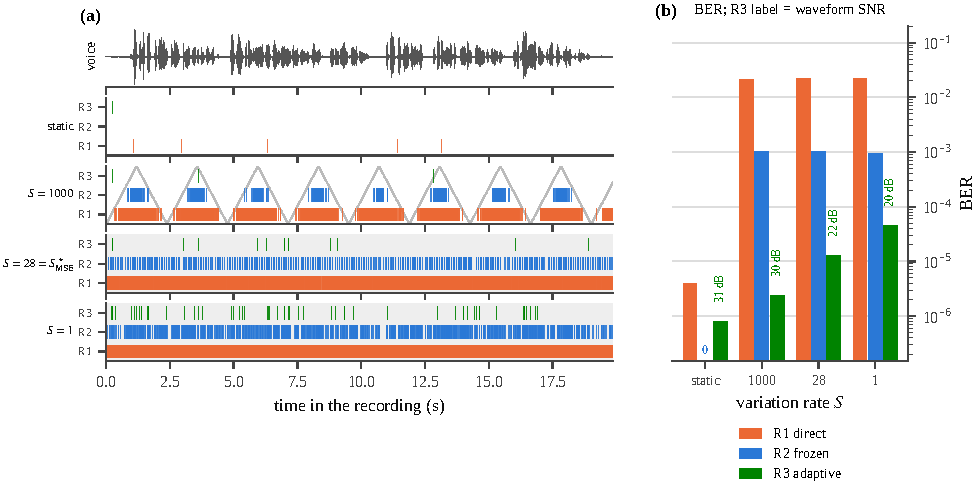
\includegraphics[width=\linewidth]{figs/audio.pdf}
\caption{Recorded voice through the time-varying primary channel, 14\,dB, $\mu=2^{-8}$, one seed (\lvl{L1}, supervised). (a)~The waveform and the position of every bit error of R1, R2 and R3 for a static channel and $S=1000$, 28 and 1 (grey: channel coefficient $a[n]$; shaded: too fast to draw). \nb{(b)~BER per receiver and scenario; R3 is labelled with its waveform SNR. At $S=1000$, R1 and R2 fail in blocks wherever $a[n]$ is large, while R3's errors stay isolated; R3 degrades gracefully from 31 to 20\,dB as the channel speeds up.}}
\label{fig:audio}
\end{figure*}

\subsection{Image payload}
\label{sec:image}
The PPR predicted that, because position in the image corresponds to elapsed time, R2 would degrade progressively down the image while R3 does not, until at fast enough variation R3 also fails. \nb{The $128\times72\times8$-bit image (a public-domain photograph shipped with scikit-image \cite{vanderwalt2014}; 5 seeds) shows both behaviours. At 14\,dB the differences are small (R2 53--90 wrong pixels, R3 0--12), so lower SNRs were run. At $S=1000$ the channel ramps once across the image and R2 degrades down the image: its BER per band of 8 rows rises from 0 to $1.4\times10^{-2}$ at 12\,dB and from $2\times10^{-5}$ to $2.5\times10^{-2}$ at 10\,dB, while R3 stays below $2\times10^{-4}$ and $1.4\times10^{-3}$ (\cref{fig:imgstats}a). R3 also fails, in both senses used here: at 10\,dB and $\mu=2^{-8}$ its BER rises from $1.4\times10^{-5}$ (static) to $1.5\times10^{-3}$ at $S=5$ and 1 (about 100 wrong pixels, 100 times its static value), and with $\mu=2^{-5}$ at $S=1$ it becomes \emph{worse than R2} (1027 against 649 wrong pixels; mean absolute pixel error 4.65 against 2.42), matching the confirmed loss of advantage in \cref{sec:p3} (\cref{fig:imggrid,fig:imgstats}b). Errors are spread evenly over the eight bit planes.} The PPR's earlier $128\times72$ result (4,911 and 380 errors) \nb{cannot be reproduced, because its channel, noise level and step size were not recorded, and is superseded by these results.}

\begin{figure}[t]
\centering
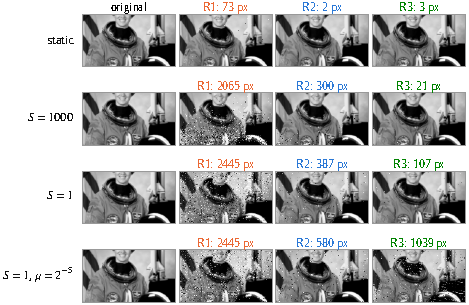
\includegraphics[width=\linewidth]{figs/image_grid.pdf}
\caption{Image payload at 10\,dB, one seed (\lvl{L1}, supervised; $\mu=2^{-8}$ unless stated). Columns: original, R1, R2, R3, with wrong-pixel counts. \nb{R2 degrades towards the bottom as the channel ramps; at $S=1$ with $\mu=2^{-5}$ R3 is worse than R2.}}
\label{fig:imggrid}
\end{figure}

\begin{figure*}[t]
\centering
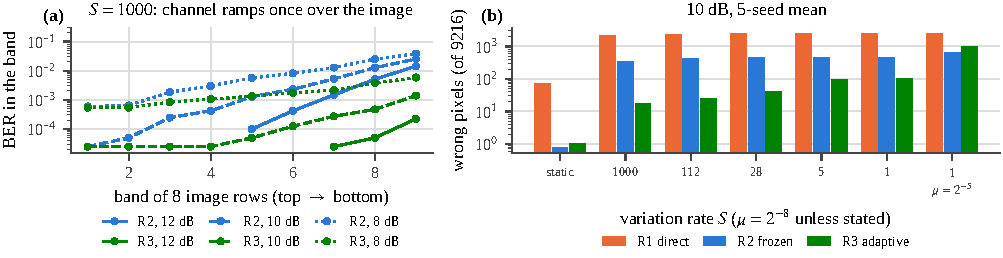
\includegraphics[width=\linewidth]{figs/image_stats.pdf}
\caption{\nb{Image payload statistics (\lvl{L1}, supervised, 5 seeds). (a)~BER per band of 8 image rows at $S=1000$, where the channel ramps once over the image: R2's BER rises down the image by two to three orders of magnitude, R3's much less. (b)~Wrong pixels at 10\,dB against the variation rate: R3 stays far below R2 until $S\approx5$, and with $\mu=2^{-5}$ at $S=1$ it is worse than R2.}}
\label{fig:imgstats}
\end{figure*}

\subsection{P6: word length against tracking (\lvl{L2})}
\label{sec:fxp}
The PPR's precision study asks how much coefficient precision is needed to sustain tracking at a given rate, with coefficient-update underflow as the expected mechanism. The bit-true model of \cref{tab:formats} uses the same LMS equations as \lvl{L1}. \nb{Four levels of agreement are kept apart: numerical equality of values, agreement of bit decisions, agreement of BER, and preservation of the tracking boundary. \emph{Equivalence:} with very wide words ($B_{\rm mul}=24$, $B_{\rm acc}=48$) the bit decisions equal \lvl{L1} (0 differences in $3.8\times10^6$); the values are not identical (MSE within $2.3\times10^{-7}$, coefficients within $4.6\times10^{-5}$) because signals are still quantised to s16.12. \emph{Static cost:} an 8-bit multiplier costs 2--9\,\% MSE, 12 and 16 bits $\le0.2$\,\%. \emph{Stalls:} the measured fraction of stalled updates matches a prediction from \lvl{L1} data (e.g.\ 0.466 against 0.489); with rounding, even 47\,\% stalled updates cost only $+0.33$\,\% MSE because the noise dithers the updates, whereas truncation biases the filter ($+31$\,\% at $\mu=2^{-11}$, 16-bit accumulator). $N_{\rm rec}$ is unchanged by word length.}

\nb{\emph{Tracking boundary against word length} (\cref{fig:fxp}; 112 configurations, all seven FPGA step sizes, 20 seeds, 16\,dB). (1)~The \emph{accumulator} width sets the boundary and the \emph{multiplier} width does not: with $B_{\rm acc}=26$, $B_{\rm mul}=8$, 12 and 16 give the same $S^\star_{\rm MSE}$ at every $\mu$, and the 8-bit multiplier costs only static accuracy (static excess 8.2/22.4\,\% against 4.5/11.5\,\% at the two channel ends, $\mu=2^{-8}$). (2)~With rounding, $B_{\rm acc}\ge16$ never moves the boundary; 14 bits move it only at $\mu=2^{-11}$, 12 bits from $2^{-8}$, 10 bits from $2^{-6}$. Smaller steps need more accumulator bits --- the underflow mechanism. (3)~Truncation needs about two more bits than rounding. \emph{Design consequence:} with round-to-nearest updates and $B_{\rm mul}=12$, a 16-bit accumulator gives the same $S^\star_{\rm MSE}$ grid point as the 26-bit baseline at all seven power-of-two step sizes, and the 26-bit row equals the \lvl{L1} boundary on the same rate grid. This is preservation of the \emph{MSE tracking boundary} (16\,dB, primary channel, 20 seeds); it does not mean that values, coefficients or BER are identical, and the BER boundary was not measured at reduced width. Using 16 rather than 26 accumulator bits is therefore a \emph{software-supported design recommendation}, not a measured saving in resources or timing.} This answers the PPR's hypothesis: \nb{underflow can restrict tracking, but only below these widths or with truncation.}

\noindent\textbf{Engineering significance.} The research question is how fast a \emph{fixed-point} LMS equalizer can track; the word-length study answers the fixed-point part. \nb{(i)~\emph{Why the accumulator matters.} Tracking is carried by many small coefficient updates $\mu e u$; each update must survive being added to the stored coefficient, so the accumulator's resolution decides whether the filter keeps moving. Smaller $\mu$ makes the updates smaller, which is why the required accumulator width grows as $\mu$ falls (\cref{fig:fxp}a). (ii)~\emph{Rounding against truncation.} Rounding loses updates below half an LSB symmetrically, and the channel noise dithers them, so the loss averages out; truncation always rounds the same way, which adds a systematic drift to every coefficient and costs about two more bits for the same boundary. (iii)~\emph{Diminishing return from the multiplier.} The multiplier width only sets how precisely the stored coefficient is used in the filter output; beyond 12 bits the output error it adds is far below the channel noise (static MSE cost $\le0.2$\,\%), and it never touches the update path, so it does not move the boundary. (iv)~\emph{What it suggests for the FPGA.} The extended-precision accumulator of the PPR can be narrower than the 26-bit baseline, with round-to-nearest, while the multiplier stays at 12 bits, within one DSP48E1 input. (v)~\emph{What it does not show.} These are \lvl{L2} results for one channel and SNR; the RTL verification, synthesis, timing and board measurements at the chosen widths are reported in \cref{sec:fpga}.}

\begin{figure*}[t]
\centering
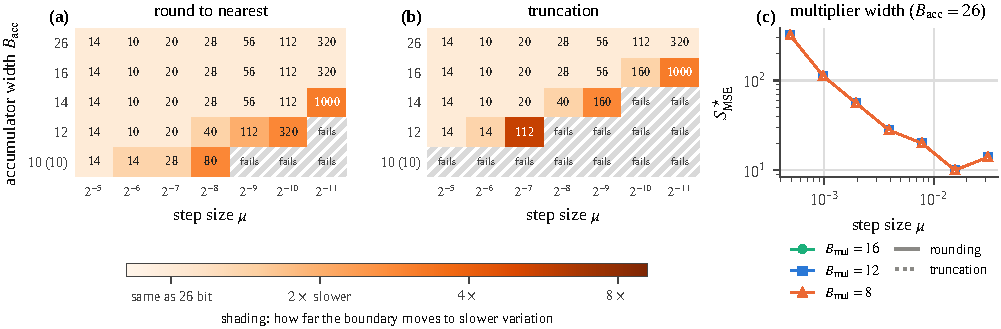
\includegraphics[width=\linewidth]{figs/fxp.pdf}
\caption{Tracking boundary $S^\star_{\rm MSE}$ against coefficient word length, primary channel, 16\,dB, 20 seeds, supervised (\lvl{L2}, bit-true; rate grid without $S=224$). \nb{(a),~(b)~Accumulator width $B_{\rm acc}$ with round-to-nearest and with truncated updates; multiplier width 12 bits (10 where shown in brackets). Each cell gives $S^\star_{\rm MSE}$; the shading shows how far the boundary moves to slower variation relative to the 26-bit row; ``fails'': the filter fails even on a static channel. (c)~Multiplier width 8, 12 and 16 bits with a 26-bit accumulator: all six curves coincide, so the multiplier does not limit tracking. With rounding, $B_{\rm acc}\ge16$ gives the same MSE boundary as 26 bits at every FPGA step size; values, coefficients and BER are not claimed identical.}}
\label{fig:fxp}
\end{figure*}

\subsection{First RTL (P7--P8, \lvl{L3})}
\label{sec:rtl}
P7--P8 were planned for the final report and started before the mid-term. Verilog exists for the 12-LFSR noise generator, the PRBS, the variation controller, the channel-plus-noise front end, R1, R2 and R3 ($L=16$; parameterised $B_{\rm mul}$, $B_{\rm acc}$, $\mu$ and rounding) and the error and MSE counters, in one chain. \nb{In iverilog simulation, the noise stream (20\,000 samples) and the full chain (7 configurations $\times$ 6000 symbols, including truncation, heavy stalling, saturation, a static and a fast ($S=1$) channel) are identical to the \lvl{L2} model in every per-symbol signal and every counter; Verilator lint reports no errors.} \nb{This behavioural code is the reference for the synthesisable rewrite of \cref{sec:fpga}, which matches it and the \lvl{L2} model bit for bit; its noise generator and PRBS are used there unchanged.}
